\section{Koordinaatisto ja funktion kuvaaja}
Funktioita reaaliluvuilta reaaliluvuille voidaan havainnollistaa koordinaatistossa kuvaajien avulla. Funktion $f$ kuvaajassa koordinaatistoon piirretään ne pisteet, joilla y-koordinaatti on $f$:n arvo sen x-koordinaatissa. Siis kaikilla $f$:n määrittelyjoukon luvuilla $x$ lasketaan $y = f(x)$ ja piirretään piste $(x, y)$ koordinaatistoon. Funktioita voi piirtää helposti myös graafisilla laskimilla tai tietokoneohjelmilla (esimerkiksi Wolfram Alphalla\footnote{\url{http://www.wolframalpha.com/}}).

% Tarvitaan kuvien ja taulukkojen vierekkäin laittamiseen.
\def\vcent#1{\mathsurround0pt$\vcenter{\hbox{#1}}$}

\begin{esimerkki}
Funktion $f(x) = \frac{x}{2} - 1$ kuvaaja sisältää kaikki pisteet $(x, y)$, joilla pätee $y = \frac{x}{2} - 1$:
\begin{center}
\begin{tabular}{cc}
\begin{tabular}{|r|l|}
\hline
$x$ & $y = f(x)$ \\
\hline
$-3$ & $-2,5$ \\
$-2$ & $-2$ \\
$-1$ & $-1,5$ \\
$0$ & $-1$ \\
$1$ & $-0,5$ \\
$2$ & $0$ \\
$3$ & $0,5$ \\
\hline
\end{tabular} &
\vcent{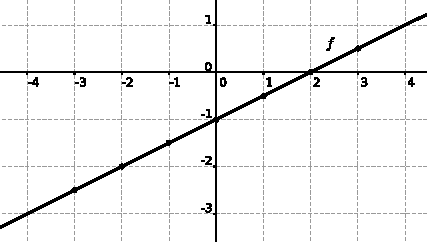
\includegraphics[width=8cm]{pictures/suoraesim.pdf}}
\end{tabular}
\end{center}
\end{esimerkki}

\begin{esimerkki}
Funktion $f(x) = x^2$ kuvaaja sisältää kaikki pisteet $(x, y)$, joilla pätee $y = x^2$:
\begin{center}
\begin{tabular}{cc}
\begin{tabular}{|r|l|}
\hline
$x$ & $y = f(x)$ \\
\hline
$-2$ & $4$ \\
$-1$ & $1$ \\
$-0,5$ & $0.25$ \\
$0$ & $0$ \\
$0,5$ & $0.25$ \\
$1$ & $1$ \\
$2$ & $4$ \\
\hline
\end{tabular} &
\vcent{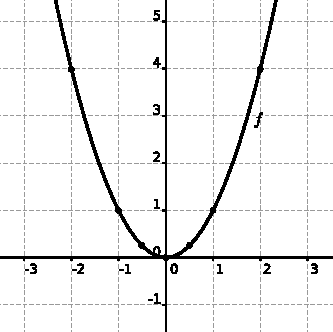
\includegraphics[width=6cm]{pictures/paraabeli.pdf}}
\end{tabular}
\end{center}
\end{esimerkki}

\begin{esimerkki}
Funktion $f(x) = x^3-5x+2$ kuvaaja sisältää kaikki pisteet $(x, y)$, joilla pätee $y = x^3-5x+2$:
\begin{center}
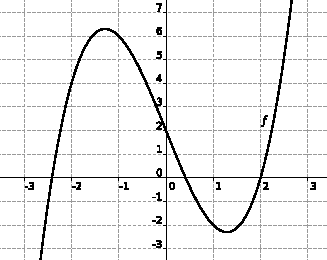
\includegraphics[width=7cm]{pictures/deg3polynomiesim.pdf}
\end{center}
\end{esimerkki}

\begin{tehtavasivu}

\paragraph*{Opi perusteet}

\begin{tehtava}
Hahmottele funktion kuvaaja kynällä ja paperilla tai laskimen avulla. Voit myös käyttää tietokonetta.
\begin{alakohdat}
\alakohta{$f(x) = 2$}
\alakohta{$f(x) = 3x+2$}
\alakohta{$f(x) = x^2$}
\alakohta{$f(x) = \frac{2}{x}$}
\end{alakohdat}

%\begin{vastaus}
%\end{vastaus}
\end{tehtava}

\begin{tehtava}
Laske taulukkoon funktion arvo pisteissä $x=-2$, $x=-1$, $x=0$, $x=1$ ja $x=2$. Hahmottele näiden tietojen avulla funktion kuvaaja.
\begin{alakohdat}
\alakohta{$f(x)= x^2+x+1$}
\alakohta{$f(x)= 3x^2$}
\alakohta{$f(x)= x^3 +2x+2$}
\end{alakohdat}
\begin{vastaus}
\begin{alakohdat}
\alakohta{$f(-2)=3,f(-1)=1, f(0)=1, f(1)=3$ ja $f(2)=7$}
\alakohta{$f(-2)=12, f(-1)=3, f(0)=0, f(1)$ ja $f(2)=12$}
\alakohta{$f(-2)=6, f(-1)=1, f(0)=2, f(1)=5$ ja $f(2)=14$}
\end{alakohdat}
\end{vastaus}
\end{tehtava}

\end{tehtavasivu}
